\jxhj{%教学后记
	}
\skrq{%授课日期
	2017年11月28日 4-5节}
\ktmq{%课题名称
	 Fanuc上的孔加工指令(二)}
\jxmb{%教学目标,每行前面要加 \item
	\item 掌握孔加工的加工工艺;
	\item 掌握Fanuc上孔加工指令的使用;
	\item 会进行孔加工程序的编写
	\item 掌握孔系的编程。}
\jxzd{%教学重点,每行前面要加 \item
	\item Fanuc上孔加工指令的使用;
	\item 孔系的编程。 }
\jxnd{%教学难点,每行前面要加 \item
	\item 孔系的编程。 }
\jjff{%教学方法
	通过讲述、举例、演示法来说明;}

\makeshouye %制作教案首页

%%%%教学内容
\subsection{组织教学}
\begin{enumerate}[\hspace{2em}1、]
	\item 集中学生注意力;
	\item 清查学生人数;
	\item 维持课堂纪律;
\end{enumerate}

\subsection{复习导入及主要内容}
\begin{enumerate}[1、]
\item Fanuc孔加工指令;
\item Fanuc 孔加工应用;
\item Fanuc 孔加工编程;
\item 编程实例。
\end{enumerate}

\subsection{教学内容及过程}
\subsubsection{一行孔的编程}
加工如图 所示六个孔Ф10,深度为30mm。
\begin{figure}[h]
	\centering
	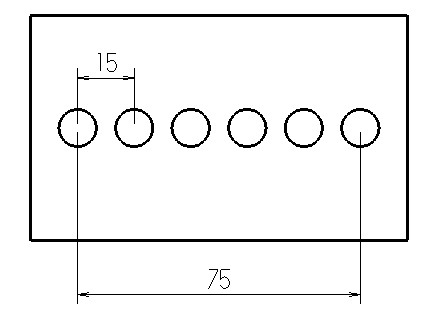
\includegraphics[width=0.7\linewidth]{data/image/22-1}
	\caption{线性均布孔实例}
	\label{fig:22-1}
\end{figure}

分析:

图中六个孔分布在同一条线上,且间距均为15mm,为了减少程序量,可以使用重复次数指令L\_\_编程。工件坐标系设置于工件上表面中心处。
加工程序如下:
\begin{lstlisting}
O21
G54G17G40G49G80
G01Z100F2000
M03S400
Z20                      
G00X-52.5Y0              定位于最左侧孔的左侧
G99G73Z-30R5Q6F80L0      定义孔加工参数的方式及相关参数
G91X15L6                 从左往右依次加工六个孔
G80
M05
M30
\end{lstlisting}

\subsubsection{一列孔的编程}
\begin{lstlisting}
O21
G54G17G40G49G80
G01Z100F2000
M03S400
Z20                      
G00X-52.5Y0              定位于最左侧孔的左侧
G99G73Z-30R5Q6F80L0      定义孔加工参数的方式及相关参数
G91Y-15L6                 从左往右依次加工六个孔
G80
M05
M30
\end{lstlisting}

\subsubsection{斜线孔系的编程}
\begin{lstlisting}
O21
G54G17G40G49G80
G01Z100F2000
M03S400
Z20                      
G00X-52.5Y0              定位于最左侧孔的左侧
G99G73Z-30R5Q6F80L0      定义孔加工参数的方式及相关参数
G91Y-15X10L6                 从左往右依次加工六个孔
G80
M05
M30
\end{lstlisting}

\subsubsection{多行孔系的编程}
\begin{lstlisting}
O21
G54G17G40G49G80
G01Z100F2000
M03S400
Z20                      
G00X-52.5Y0              定位于最左侧孔的左侧
M98 P10 L10                从左往右依次加工六个孔
G80
M05
M30

O10
G99G73Z-30R5Q6F80L0      定义孔加工参数的方式及相关参数
G91X15L6 
G1X-15Y10
M99
\end{lstlisting}


\subsection{课堂小结}
\begin{enumerate}[1、]
\item 一行孔的编程;
\item 一列孔的编程;
\item 斜线孔系的编程;
\item 多行孔系的编程。
\end{enumerate}

\vfill
\subsection{布置作业}
\begin{enumerate}[1、]
	\item 综合习题一。
\end{enumerate}
\vfill